\lab{Algorithm}{Pseudorandom Number Generators}{Pseudorandom Number Generators}
\label{Ch:PRNG}

\objective{Teach how to build pseudorandom number generators and the differences between the different kinds of pseudorandom number generators}

\section*{Random Numbers}

Lotteries, most board games, and statistics need random numbers.
In real life, we roll dice, take balls out of a bag, or spin a wheel.
Computers are, by nature, deterministic, meaning that they do exactly what they are told.
Because of this, random number generation on a computer can be difficult.
We can have a device measure a random process and use the data to generate random numbers, 
But such sampling is often too slow and too expensive for practical use.
Pseudorandom number generators (PRNGs) are a common solution to this problem.
The numbers are not truly random, but they are based on a complex formula that makes them look ``random."
For convenient use, these generateors must also run quickly.
The goal is to have something that is fast and looks random.

There are many different algorithms for developing pseudorandom numbers.
Robert R. Coveyou titled an article ``The generation of random numbers is too important to be left to chance."
There has been much study about different PRNGs.
This lab will cover two of them: Linear Congruiental Generators and The Mersenne Twister.

\section*{Linear Congruential Genterators}

Linear Congruential Generators (LCG) are one of the oldest ways of generating random numbers.
The Generator is defined by the recurrence relation:
$X_{n+1}=(a*X_n + c)$ mod $m$ where

\begin{itemize}
\item $X$ is a sequence of pseudorandom values, and
\item $m$, $0<m$ is the modulus
\item $a$, $0<a<m$ is the multiplier
\item $c$, $0\leq c<m$ is the increment
\item $X_0$, $0\leq X_0 <m$ is the seed
\end{itemize}

each of these are integer constants.

\begin{problem}
Write a LCG that produces an array of pseudorandom numbers between $0.0$ and $1.0$.
Let the arguments be size of the array and let a, c, mod, and seed be optional arguments.
I recommend $a=1103515245$, $c=12345$, $m=2^{31}-1$, and $seed=4329$ as the default values.
\end{problem}

\begin{problem}
Write a LCG that produces an array of pseudorandom numbers of integers between two input arguments.
Do it by calling your algorithm from problem one and multiplying it by the values and casting the array as an int using the .astype() function.
Let the arguments be size of array and the two integers.
Let a, c, mod, and seed continue to be optional arguments.
\end{problem}

One easy way to ``see" if your generator is random is to look at a bitmap of the output.
In python, use the plt.imshow() function to see a bitmap of the array produced by your LCG.
Resize your output to be $512 \times 512$.

\begin{figure}[H]
%\begin{center}
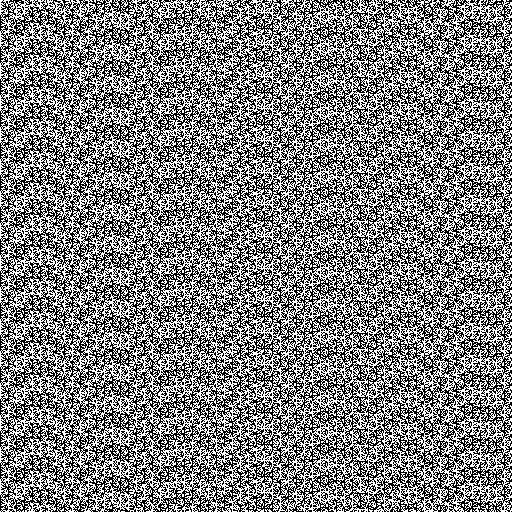
\includegraphics[scale = .4]{PRNG1.jpg}
\caption{
The bitmap with $a=25214903917$, $c=11$, $m=2^{48}$.
There is a clear pattern in the random numbers.}
%\end{center}
\end{figure}

\begin{problem}
For what values of $a$, $c$, and $m$ does your LCG have a visible pattern.
\end{problem}

This method is not rigorous, but there are several other ways to test the randomness of your output.

The length over which your random number generator repeats is called the period.
The period is at most m, but it may be shorter based on the values of a and c.
 
According to the Hull-Dobell Theorem (TO DO: find a source), a LCG will have a full period if and only if, 
1. $c$ and $m$ are relatively prime,
2. $a-1$ is divisible by all prime factors of $m$,
3. $a-1$ is a multiple of 4 if $m$ is a multiple of 4

\begin{problem}
Test values of $a$,$c$, and $m$ that fit these requirements. 
\end{problem}

This algorithm is used as the default random number generator in Java, and C++ and is still used in a wide variety of situations.

\section*{Mersenne Twister and Bitwise operations}

(TO DO: decide how much of  this we want to keep) All numbers can be represented in bits as a base two number.
Computers are optimized to work with numbers in that manner.
The operators XOR, OR, and AND work on the bit representation of two numbers.

AND - if both numbers have a 1 in the ith place then the ith place is 1.
Otherwise the ith place is 0.

OR - if one or both numbers have a 1 in the ith place then the ith place is 1.
Otherwise the ith place is 0.

XOR - if only one of the two numbers has a 1 in the ith place then the ith place is 1.
If both or neither of the numbers has a 1 in the ith place, the ith place is 0.

In addition you can shift the bitwise number over a number of values.
For example, shifting 10100 to the right by one yields 1010 and shifting it to the left by one yields 101000.
This is really just division and multiplication by 2.
This can be done by $\ll$ and $\gg$ in python. 

The Mersenne twister PRNG does a series of these operations to generate random numbers.
The Random class in python uses the Mersenne twister algorithm. 

\begin{problem}
Look at the bitmap of output of sp.rand(512,512).
Can you see any patterns?
\end{problem}

\begin{problem}
Analyze the first of 10,000 outputs of the random class.
Can you see a period?
\end{problem}
